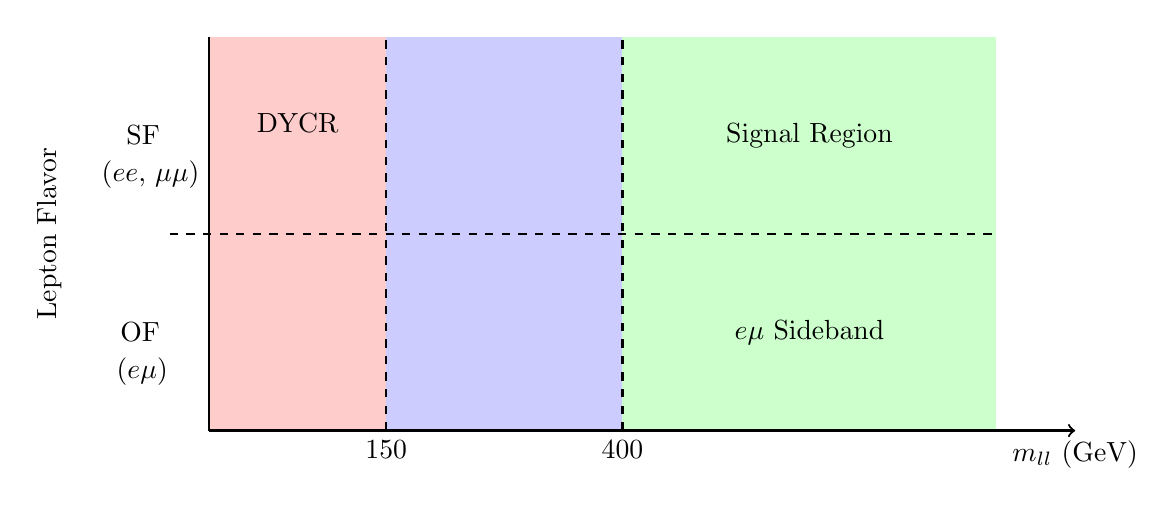
\begin{tikzpicture}[scale=5]
  
    % Define the division points for the three regions
    \def\xone{0.45}   % Right boundary of region 1 (SR)
    \def\xtwo{1.05}   % Right boundary of region 2 (CR) / left boundary of region 3 (SB)
    \def\xmax{2}      % Overall width of the box
    
    % Draw and fill the three vertical regions
    \fill [red!20!white]      % Region 1: SR
      (0,0) rectangle (\xone,1);
    \fill [blue!20!white]     % Region 2: CR (Control or Central Region)
      (\xone,0) rectangle (\xtwo,1);
    \fill [green!20!white]    % Region 3: SB
      (\xtwo,0) rectangle (\xmax,1);
      
    % Draw dashed vertical division lines for the three regions
    \draw[dashed,thick] (\xone,0) -- (\xone,1);
    \draw[dashed,thick] (\xtwo,0) -- (\xtwo,1);
    
    % Draw a horizontal dashed line at y = 0.5 (dividing OS and SS regions)
    \draw[dashed,thick] (-0.1,0.5) -- (\xmax,0.5);
    
    % Label the y-axis regions (lepton charges)
    \draw
      (-0.1,0.75) node[anchor=east] {SF}
      (0,0.65) node[anchor=east] {($ee$, $\mu\mu$)}
      (-0.1,0.25) node[anchor=east] {OF}
      (-0.08,0.15) node[anchor=east] {($e\mu$)};
    
    % Label the x-axis regions (lepton isolations)
    \draw
      (\xone,0) node[anchor=north] {150}
      (\xtwo,0) node[anchor=north] {400};
    
    % Add axis descriptions (the Lepton Flavor label remains on the left)
    \draw
      (-0.35,0.5) node[rotate=90,anchor=south] {Lepton Flavor};
    
    % Draw the x-axis as an arrow along the bottom edge.
    \draw[->, thick] (0,0) -- (\xmax+0.2,0) node[anchor=north] {$m_{ll}$ (GeV)};
    \draw[thick] (0,0) -- (0,1) node[anchor=west] {};

    % Add internal region labels (adjust positions as needed)
    \draw
      (\xone/2,0.78) node {DYCR}
      ({\xtwo + (\xmax-\xtwo)/2},0.25) node[align=center] {$e\mu$ Sideband}
      ({\xtwo + (\xmax-\xtwo)/2},0.75) node[align=center] {Signal Region};
    
\end{tikzpicture}